 \documentclass{beamer}
\usepackage[utf8]{inputenc}
\usepackage{verbatim}
\usepackage{minted}
\usepackage[spanish]{babel}
\usetheme{Frankfurt}
\usecolortheme{seahorse}
\useoutertheme{shadow}
\useinnertheme{circles}
\graphicspath{ {./figures/} }
\title[Laboratorio]{Herramientas de trabajo (2)}
\author[Miguel]{Miguel Angel Piña Avelino}
\institute[UNAM]{
  Ingeniería de Software,\\
  Facultad de Ciencias, UNAM
}
\AtBeginSection[]{
  \begin{frame}
  \vfill
  \centering
  \begin{beamercolorbox}[sep=8pt,center,shadow=true,rounded=true]{title}
    \usebeamerfont{title}\insertsectionhead\par%
  \end{beamercolorbox}
  \vfill
  \end{frame}
}


\date{\today}
\begin{document}

\frame{\titlepage}
\begin{frame}
  \frametitle{Índice}
  \tableofcontents
\end{frame}

\section{¿Cómo funciona una aplicación web?}

\begin{frame}
  \frametitle{Conceptos}
  \begin{itemize}[<+->]
  \item HTTP
  \item Ciclo de vida de una petición HTTP
  \item Servlet
  \item Ciclo de vida de un servlet
  \end{itemize}
\end{frame}

\begin{frame}
  \frametitle{¿Qué es HTTP?}
  Protocolo de comunicación que permite las transferencias de
  información en la Internet.
  \begin{itemize}[<+->]
  \item Orientado a transacciones
  \item Esquema cliente servidor
  \item El cliente (user agent) realiza una petición enviando un
    mensaje con cierto formato al servidor.
  \item El servidor envía un mensaje de respuesta (información).
  \end{itemize}
\end{frame}

\begin{frame}
  \frametitle{Métodos de petición}
  \begin{itemize}[<+->]
    \item Define una serie predefinida de métodos de petición (algunas
      veces referido como ``verbos'') que pueden utilizarse.
    \item Tiene flexibilidad para ir añadiendo nuevos métodos.
    \item Cada método indica la acción que desea que se efectúe sobre el recurso
      identificado.
  \end{itemize}
\end{frame}

\begin{frame}
  \frametitle{Métodos de petición}
  \textbf{HEAD}\\
  Pide una respuesta idéntica a la que correspondería a una petición
  GET, pero en la respuesta no se devuelve el cuerpo. Esto es útil
  para poder recuperar los metadatos de los encabezados de respuesta,
  sin tener que transportar todo el contenido.
\end{frame}

\begin{frame}[fragile]
  \frametitle{Métodos de petición}
  \textbf{GET}\\
  Pide una representación del recurso especificado. Por seguridad no
  debería ser usado por aplicaciones que causen efectos ya que
  transmite información a través de la URI agregando parámetros a la
  URL.\@ La petición puede ser simple, es decir en una línea o compuesta.
\end{frame}

\begin{frame}[fragile]
  \frametitle{Métodos de petición}
  Ejemplo:
\begin{minted}[fontsize=\scriptsize]{python}
  http GET
  https://upload.wikimedia.org/wikipedia/commons/d/dd/Zkip_alibaba1.png
\end{minted}
obtiene un recurso llamado Zkip\_alibaba1.png\\
Ejemplo con parámetros:
\begin{minted}[fontsize=\scriptsize]{python}
http GET http://html.net/tutorials/php/lesson10_ex1.php?name=Joe
http GET http://html.net/tutorials/php/lesson10_ex1.php
\end{minted}

\end{frame}

\begin{frame}
  \frametitle{Métodos de petición}
  \textbf{POST}\\
Envía los datos para que sean procesados por el recurso
identificado. Los datos se incluirán en el cuerpo de la
petición. Esto puede resultar en la creación de un nuevo recurso o de
las actualizaciones de los recursos existentes o ambas
cosas. Generalmente es usando para enviar datos a través de
formularios.
\end{frame}

\begin{frame}
  \frametitle{Métodos de petición}
  Existen otros métodos que están dentro del protocolo HTTP, pero no
  ahondaremos en su funcionamiento, pero si mencionaremos cuales son:

  \begin{itemize}
  \item PUT
  \item DELETE
  \item TRACE
  \item OPTIONS
  \item CONNECT
  \item PATCH
  \end{itemize}
\end{frame}

\begin{frame}[fragile]
  \frametitle{Métodos de petición}
  \begin{figure}[ht]
    \centering
    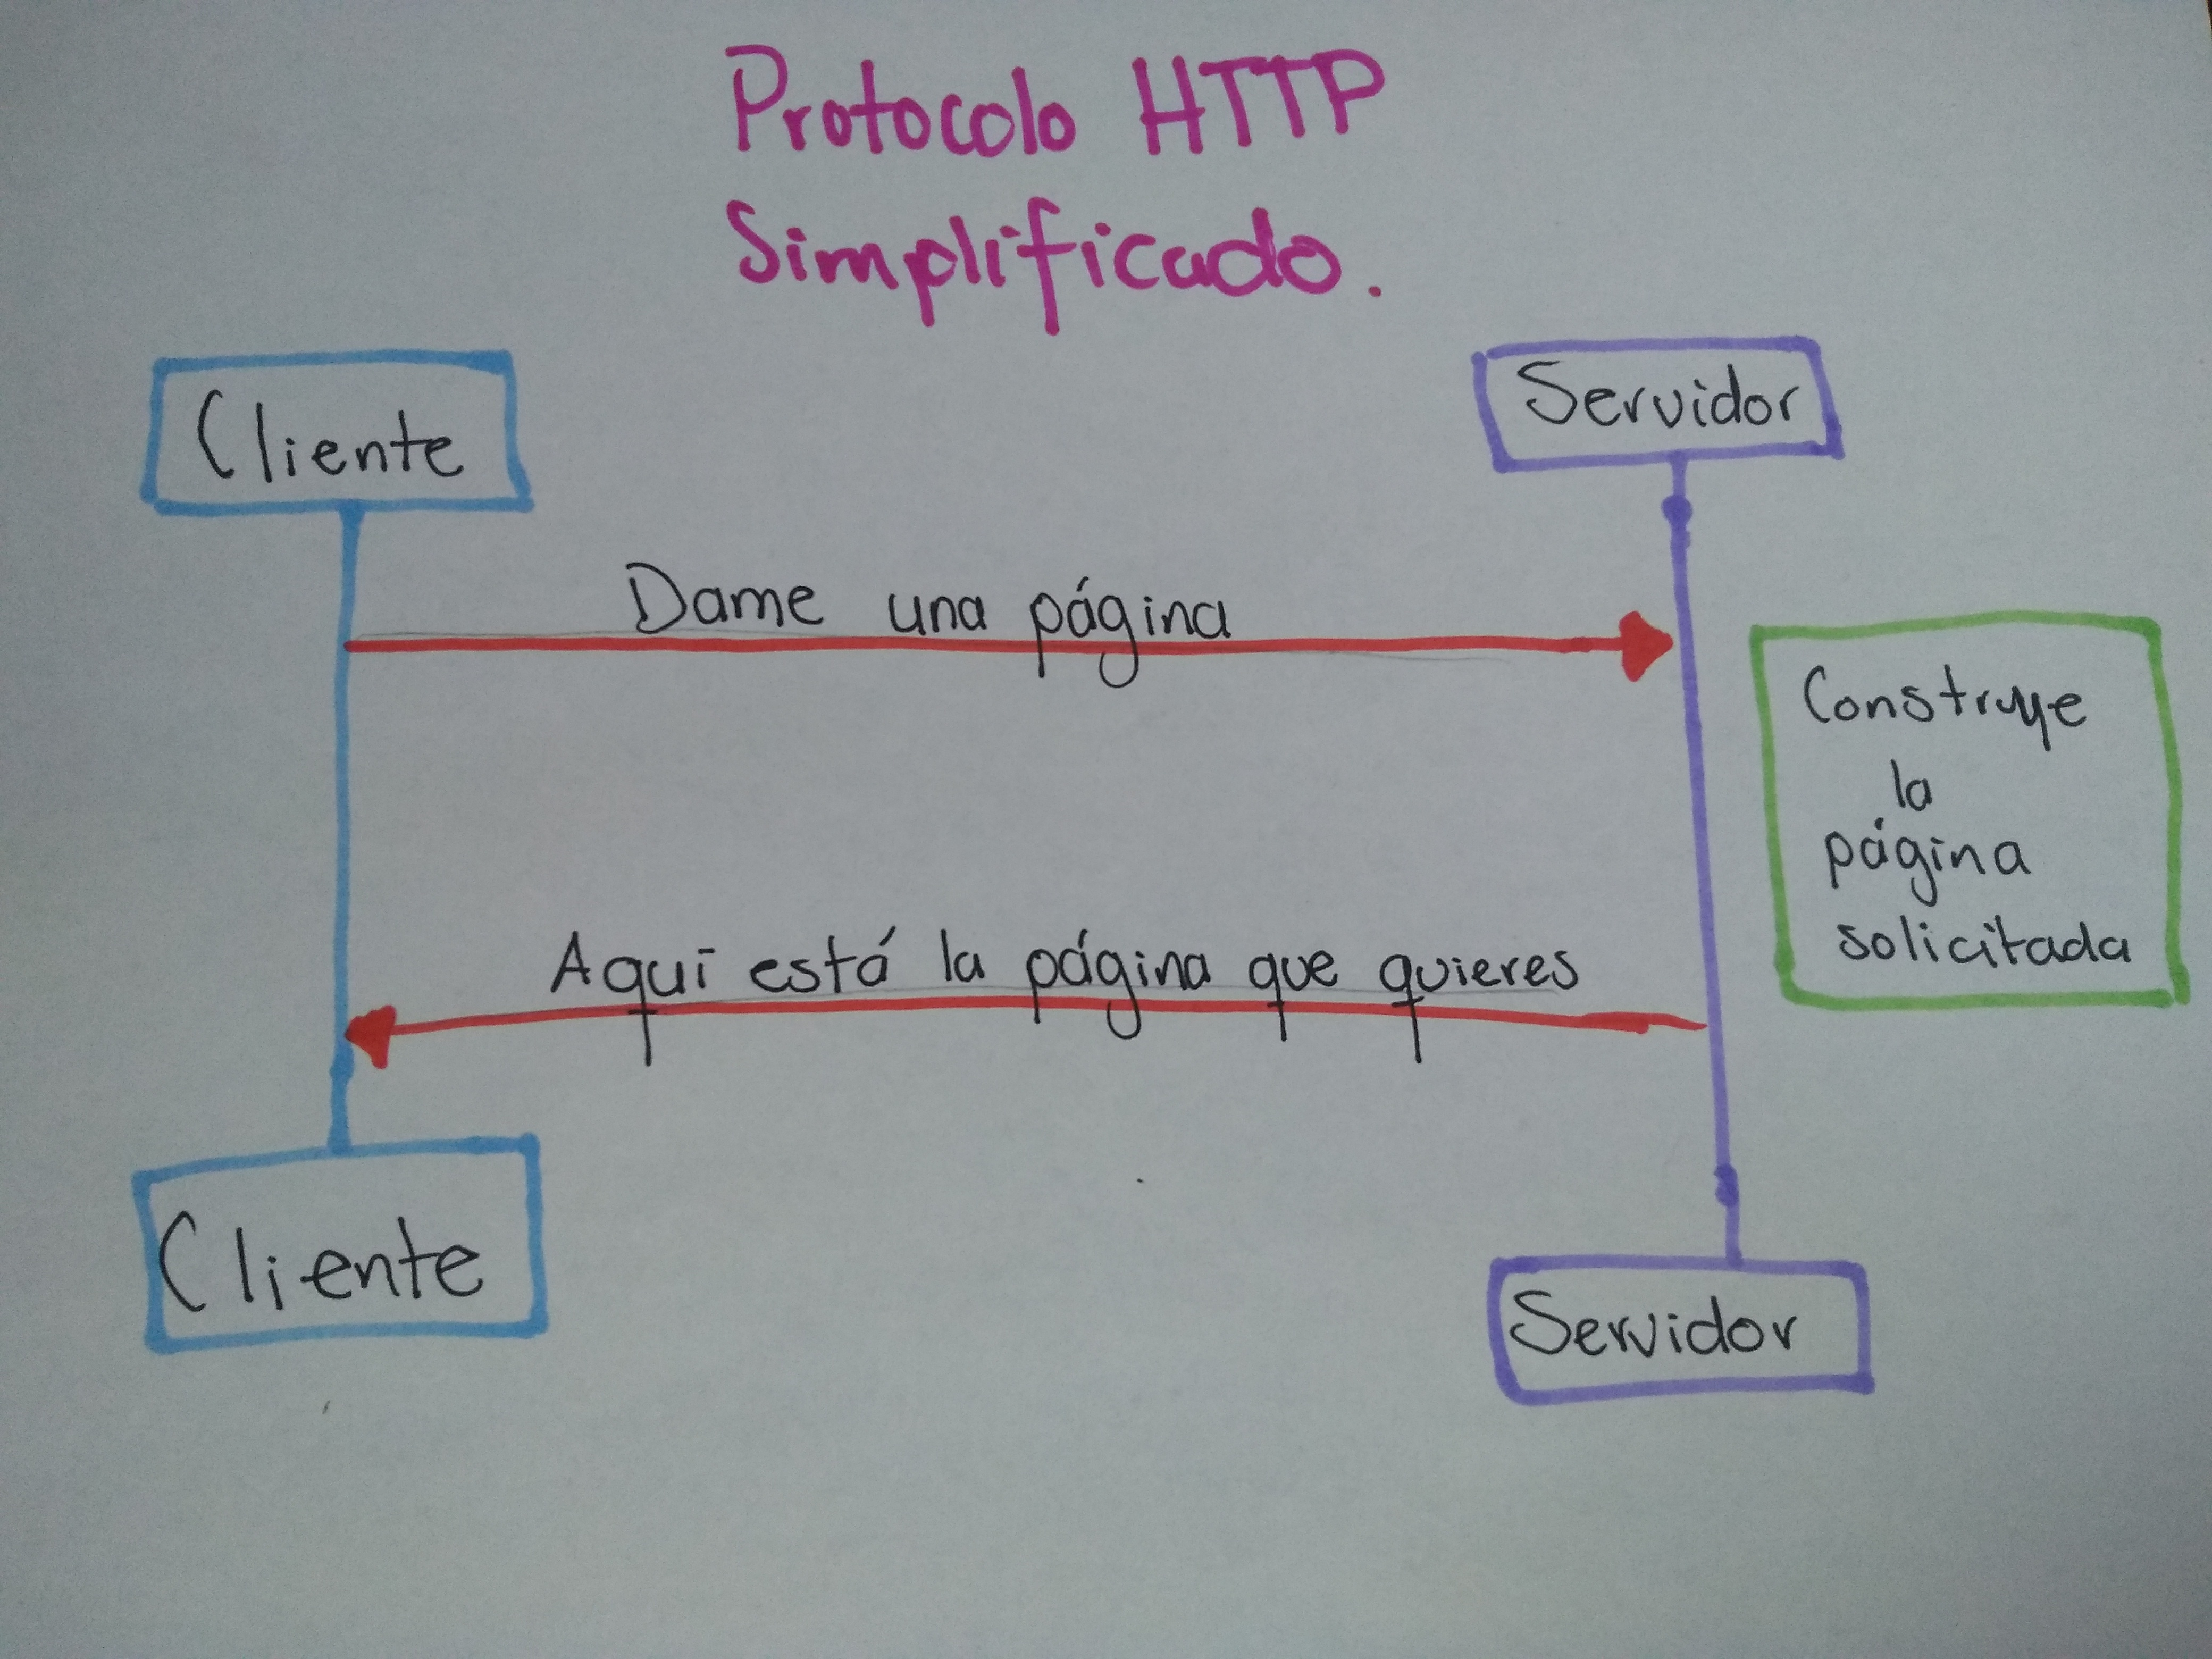
\includegraphics[scale=0.05]{figures/image01.jpg}
    \caption{\label{fig:img01} Protocolo HTTP simplificado}
  \end{figure}
\end{frame}

\section{Ciclo de vida de peticiones a servidores Java}

\begin{frame}[fragile]
  \frametitle{Ciclo de vida de peticiones JSP}
  \begin{figure}[ht]
    \centering
    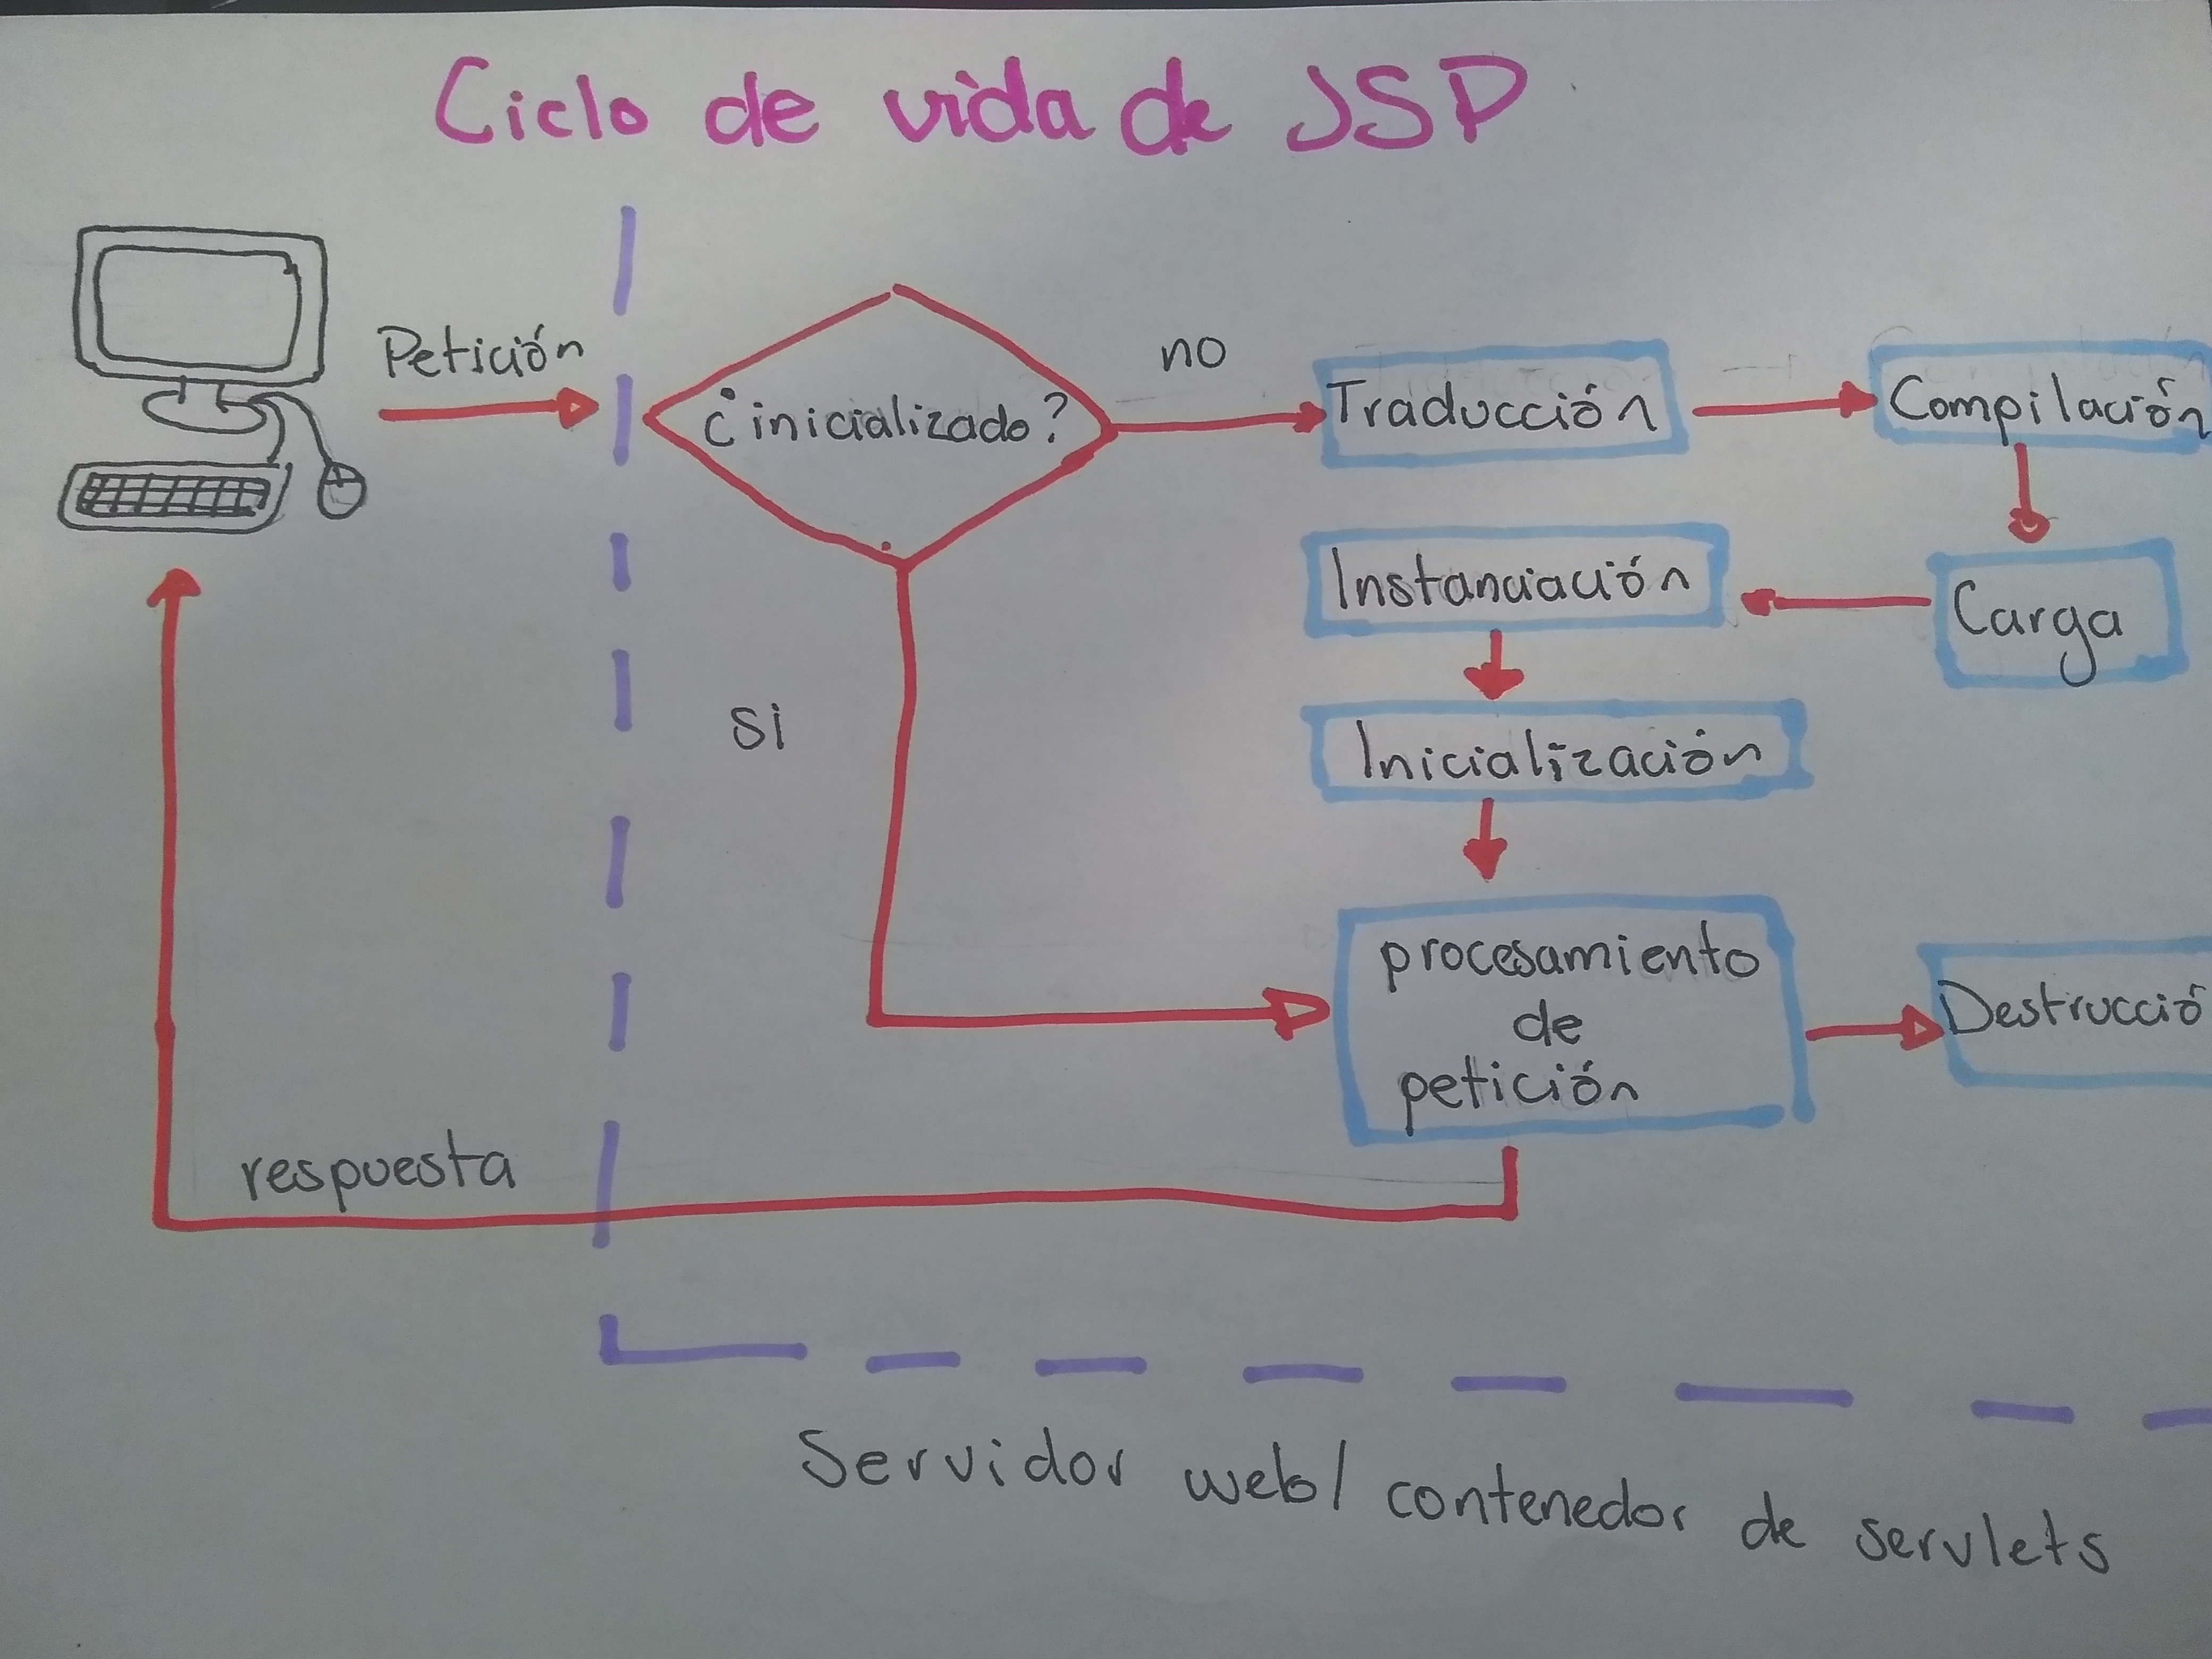
\includegraphics[scale=0.05]{figures/image02.jpg}
    \caption{\label{fig:img02} Ciclo de vida de un JSP}
  \end{figure}
\end{frame}

\begin{frame}[fragile]
  \frametitle{Ciclo de vida de un Servlet}
  \begin{figure}[ht]
    \centering
    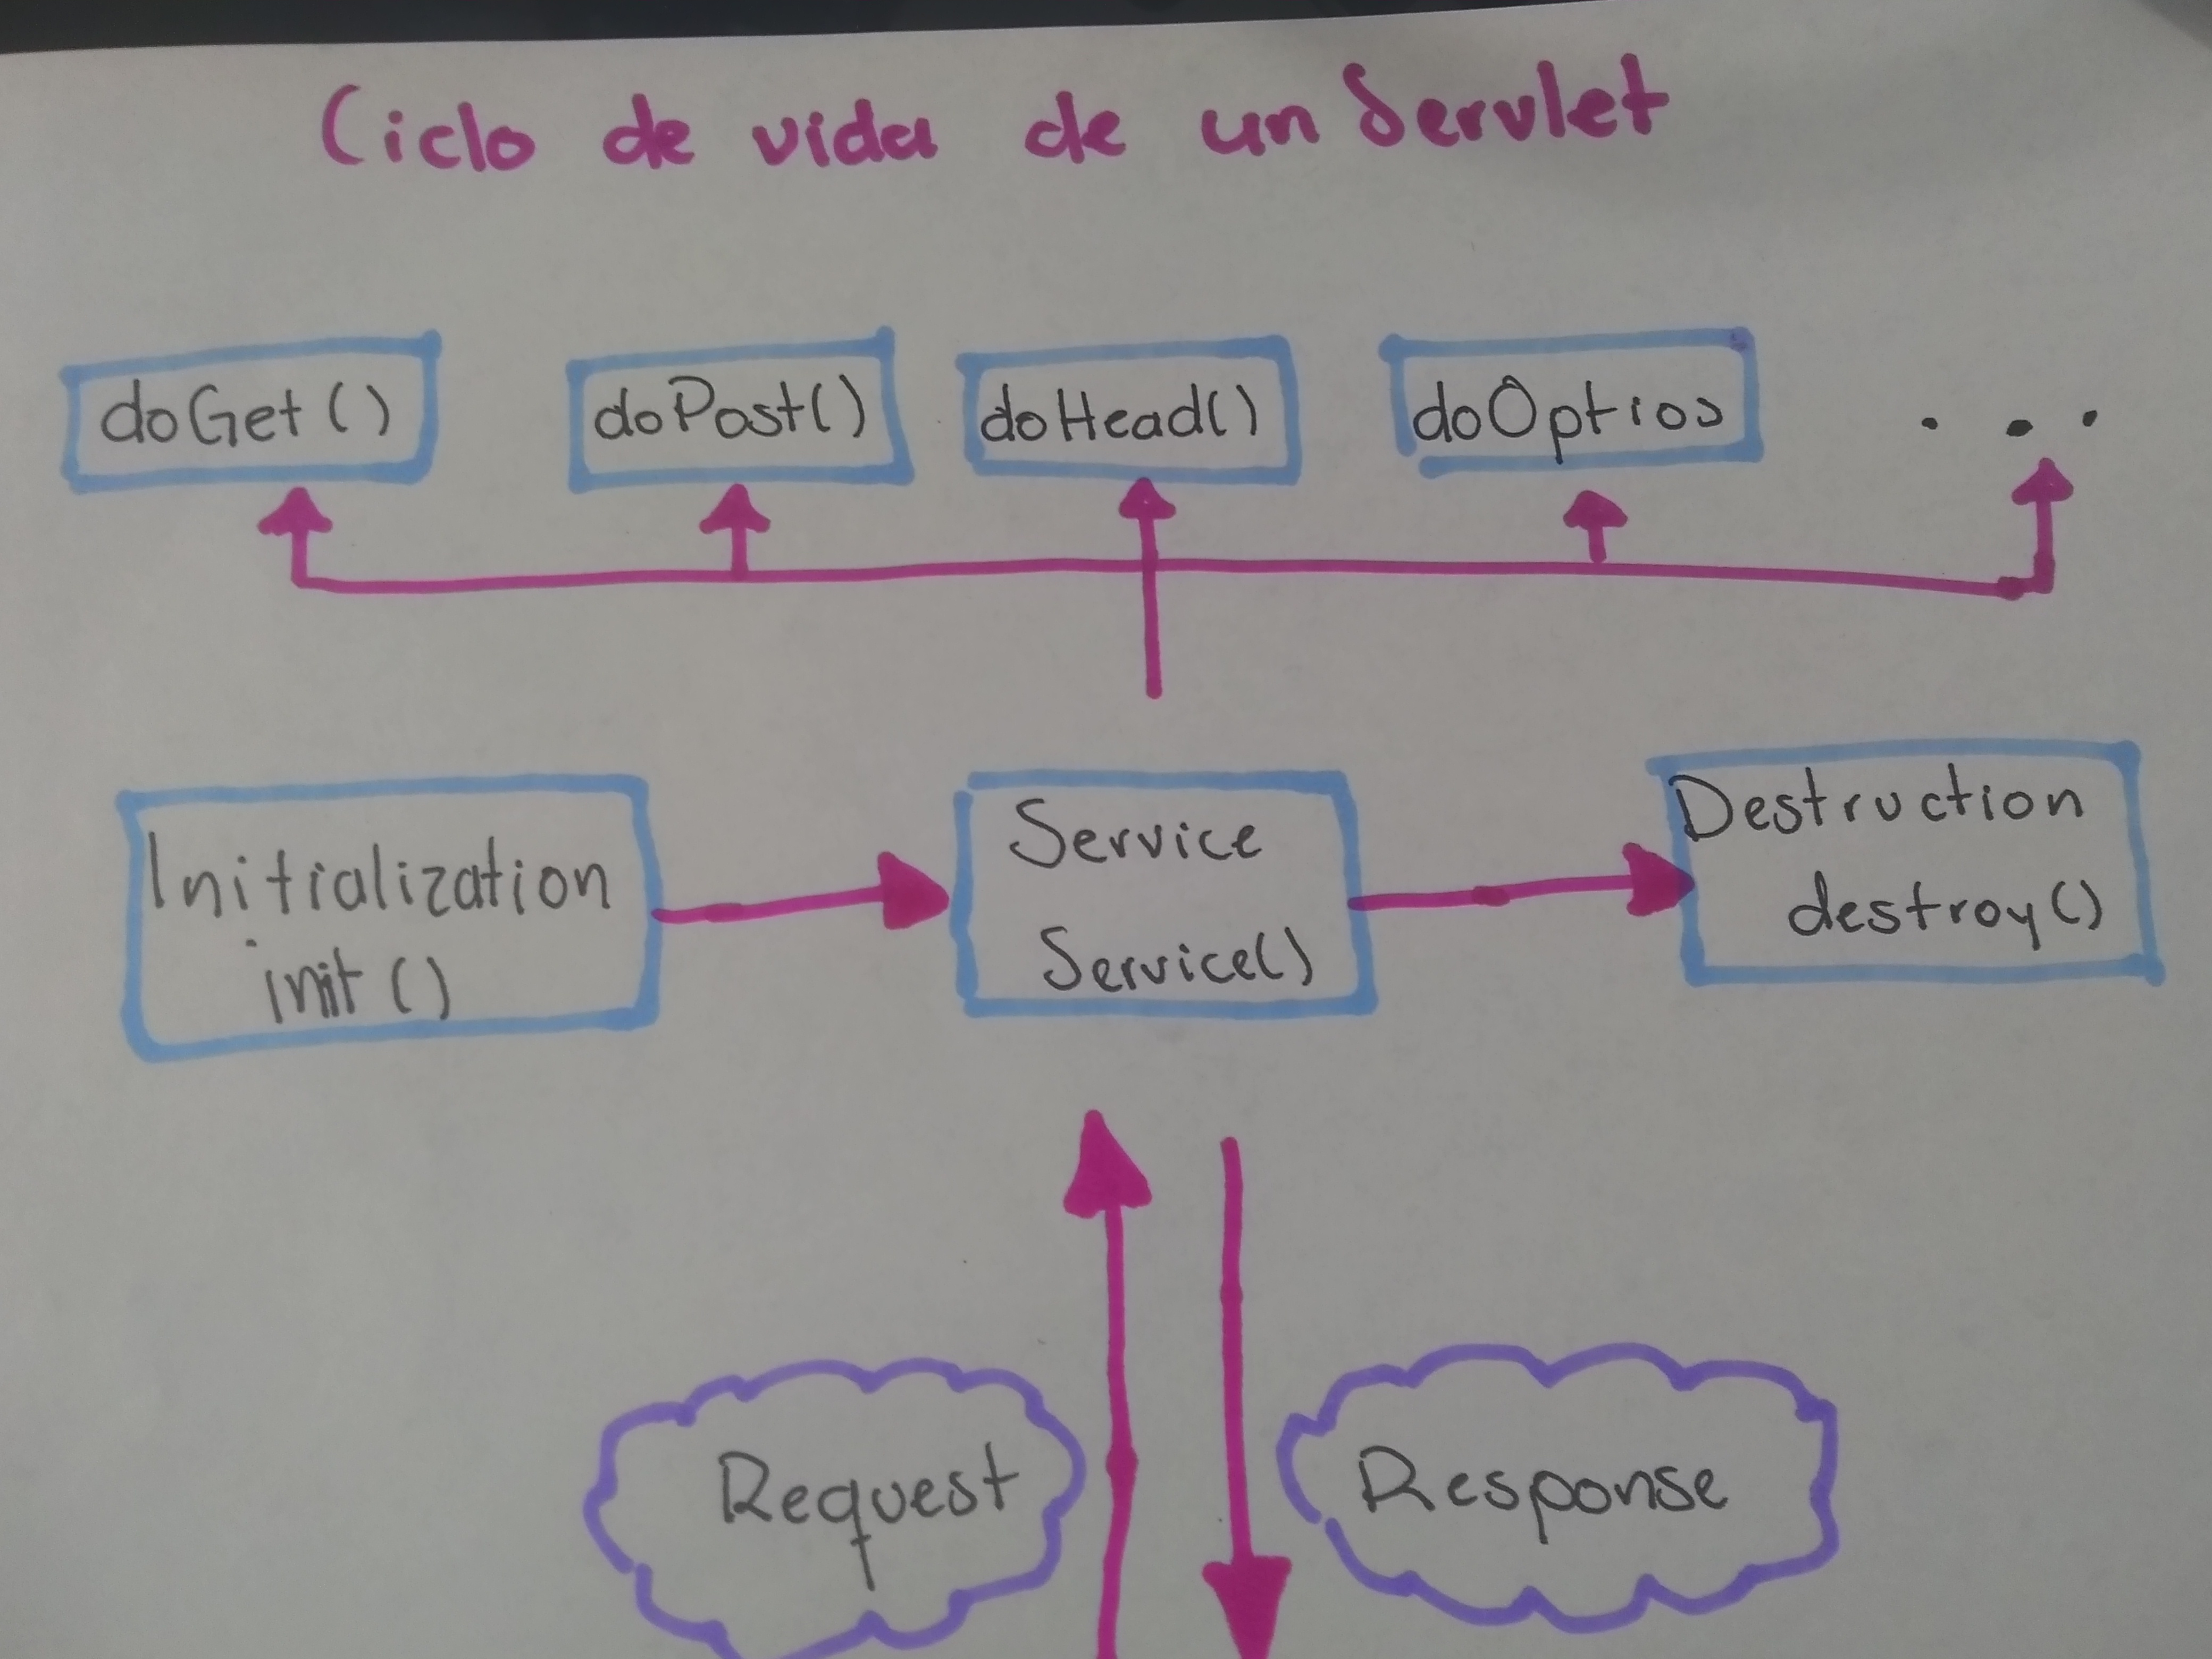
\includegraphics[scale=0.05]{figures/image03.jpg}
    \caption{\label{fig:img03} Ciclo de vida de un Servlet}
  \end{figure}
\end{frame}

\section{Sistemas de control de versiones (Git)}

\begin{frame}
  \frametitle{Sistemas de control de versiones}
  \begin{itemize}[<+->]
  \item Un sistema de control de versiones, es un sistema de software
    que permite llevar el registro y la gestión de los cambios que se dan
    sobre los elementos de algún producto.
  \item Una versión, revisión o edición de un producto, es el estado
    en el que se encuentra el mismo en un momento dado de su desarrollo o
    modificación.
  \item El control de versiones se realiza principalmente dentro del
    desarrollo de software para controlar las distintas versiones del
    código fuente dando lugar a los sistemas de control de código fuente.
  \end{itemize}
\end{frame}

\begin{frame}
  \frametitle{¿Por qué necesito uno?}
  \begin{itemize}[<+->]
  \item Es necesario llevar un control de los distintos tipos de
    cambios que se realizan sobre el código que implementamos.
  \item Además, si estamos trabajando de forma colaborativa, también
    es necesario llevar un registro de quien o quienes implementaron
    alguna características, el por qué se implementó de cierto modo, etc.
  \item Además permite llevar el código a un estado anterior sin
    perder la información más reciente.
  \end{itemize}
\end{frame}

\begin{frame}
  \frametitle{¿Qué Sistemas de Control de Versiones existen?}
  Los sistemas de control de versiones más populares en este momento
  son:
  \begin{itemize}
    \item Subversión (Svn)
    \item git
    \item Mercurial
  \end{itemize}
  En este curso vamos a utilizar git como \textbf{SCV}.
\end{frame}

\begin{frame}[fragile]
  \frametitle{¿Cómo obtener Git?}
  La última versión\footnote[frame]{Se recomienda que todos los
    integrantes del equipo tengan la misma versión instalada.} de
  \textbf{Git} se puede obtener desde la página:
  \begin{verbatim}
   https://git-scm.com/
  \end{verbatim}
\end{frame}

\begin{frame}
  \frametitle{¿Qué es Git?}
  \begin{itemize}[<+->]
    \item GIT es un software de control de versiones diseñado por
      Linus Torvalds, pensando en la eficiencia y la confiabilidad del
      mantenimiento de versiones de aplicaciones cuando estas tienen un gran
      número de archivos de código fuente.
    \item Git surge como alternativa a BitKeeper, un control de
      versiones privativo que usaba en ese entonces para el kernel.
    \item Es liberado bajo una licencia GNU GPLv2 y se ha convertido
      en uno de los más usados alrededor del mundo.
  \end{itemize}
\end{frame}

\section{Usando Git}

\begin{frame}[fragile]
  \frametitle{Inicializando Git}
  Para usar git, hay que crear una carpeta donde vamos a llevar el
  control de versiones de nuestro código, vamos a hacer lo siguiente:  \\

  \begin{minted}[fontsize=\scriptsize]{sh}
$ mkdir mi-proyecto  # Creamos una carpeta para el proyecto
$ cd mi-proyecto     # Nos movemos a esa carpeta
$ git init           # Inicializamos el repositorio
\end{minted}
\end{frame}

\begin{frame}[fragile]
  \frametitle{Checando el estado del proyecto}
  La forma en que inicializamos nuestro proyecto con gil, es a través
  de la instrucción \texttt{git init}. Una vez inicializado el proyecto,
  procedemos a revisar el estado del repositorio con \texttt{git status}.\\

  \begin{minted}[fontsize=\scriptsize]{sh}
$ git status # Checa el estado de los archivos en el repositorio
  \end{minted}
\end{frame}

\begin{frame}[fragile]
  \frametitle{Agregando archivos y haciendo commit}
  He creado un archivo llamado README.org que va a contener la
  descripción del proyecto. Por ejemplo, tendría algo como lo
  siguiente:

  \begin{minted}[fontsize=\scriptsize]{sh}
#+title: Mi proyecto
#+author: Miguel Piña
#+date: [2017-02-19 dom 19:36]

Es es un ejemplo de descripción para mi primer proyecto en git. Seguro
contendrá el modo de uso y un proyecto en maven.

* ¿Cómo compilar el proyecto?
** Como configurar la base de datos para que compile el proyecto
** ¿Qué dependencias son necesarias?
* Estilo de codificación
* Gotchas
  \end{minted}
\end{frame}


\begin{frame}[fragile]
  \frametitle{Agregando archivos y haciendo commit}
  Para agregar este primer archivo a nuestro proyecto, vamos a realizar lo
siguiente: \\

\begin{minted}[fontsize=\scriptsize]{sh}
$ git add README.org
$ git status
\end{minted}

La forma de hacer el commit de una modificación y que quede registrada
es con la instrucción \texttt{git commit}. Existe una variante en la
que se puede agregar un mensaje directamente sin tener que abrir el
editor de texto: \texttt{git commit -m ``Agregando el README''}, pero
esta no la vamos utilizar en este momento.
\end{frame}

\begin{frame}[fragile]
  \frametitle{Agregando archivos y haciendo commit}

  Ejecutamos el comando:\\

  \begin{minted}[fontsize=\scriptsize]{sh}
$ git commit
  \end{minted}

Los pasos anteriores se puede repetir tantas veces como sea
necesario. Existen herramientas que facilitan estos pasos en Netbeans
como en Emacs. La primera viene integrada dentro de Netbeans y la
segunda como un plugin llamado \texttt{magit}.
\end{frame}

\begin{frame}[fragile]
  \frametitle{Viendo el historial de cambios}

  Para ver la lista de cambios que tiene un proyecto dado, es posible usar la
siguiente instrucción:

\begin{minted}[fontsize=\scriptsize]{sh}
$ git log
\end{minted}

También se puede agrega una variante para que sea posible verla en forma de
grafo dentro de la terminal:

\begin{minted}[fontsize=\scriptsize]{sh}
$ git log --graph --decorate --pretty=oneline --abbrev-commit
\end{minted}

La sentencia anterior se puede agregar a un alias dentro de un archivo de
configuración \texttt{~/.gitconfig}, a algo como:

\begin{minted}[fontsize=\scriptsize]{sh}
[alias]
    tree = log --graph --decorate --pretty=oneline --abbrev-commit
\end{minted}

Y se puede invocar como:

\begin{minted}[fontsize=\scriptsize]{sh}
$ git tree
\end{minted}

\end{frame}


\begin{frame}[fragile]
  \frametitle{Agregando repositorios remotos}
  Hay que crear un repositorio remoto (en \textit{github}) y agregamos la
  siguiente instrucción:

\begin{minted}[fontsize=\scriptsize]{sh}
$ git remote add origin https://github.com/miguelpinia/something.git
\end{minted}

Hay que remplazar la url por la del repositorio. Una vez agregado el repositorio
remoto, hay que empujar todos los cambios que hemos hecho en nuestro repositorio
local:

\begin{minted}[fontsize=\scriptsize]{sh}
git push -u origin master
\end{minted}

\end{frame}

\begin{frame}[fragile]
  \frametitle{Obteniendo cambios desde repositorio}

  Supongamos que alguien hizo cambios en el repositorio y los empujó al
repositorio, para obtener esos cambios, ejecutamos la instrucción:

\begin{minted}[fontsize=\scriptsize]{sh}
$ git pull
\end{minted}

Para ver cuales fueron los cambios que se hicieron entre el último commit que
teníamos y el que obtuvimos ejecutamos:

\begin{minted}[fontsize=\scriptsize]{sh}
$ git diff HEAD
\end{minted}

\end{frame}

\begin{frame}[fragile]
  \frametitle{Creando ramas}
  Para agregar cambios sin modificar el contenido de la rama principal
  (rama master), vamos a crear una nueva rama donde podamos
  trabajar. Para hacer esto, realizamos lo siguiente:

\begin{minted}[fontsize=\scriptsize]{sh}
$ git checkout -b mi_nueva_rama
\end{minted}

A partir de aquí podemos realizar nuevos cambios. Para regresar o
moverse entre ramas, usando el comando checkout sin banderas.

\begin{minted}[fontsize=\scriptsize]{sh}
$ git checkout master
\end{minted}

\end{frame}

\begin{frame}[fragile]
  \frametitle{Mezclando ramas}
  Después de realizar una serie de cambios, es necesario que se mezclen con la
rama principal. Una forma limpia de hacerlo, es haciendo un rebase de la rama
con la que estamos trabajando respecto a la que vamos a mezclar.
\end{frame}

\begin{frame}[fragile]
  \frametitle{Mezclando ramas}
  La acción de rebase, se refiere a desplazar todos los cambios que
  existan en la rama a mezclar y que no se han integrado con la rama que
  estamos trabajando.

\begin{minted}[fontsize=\scriptsize]{sh}
$ git checkout mi_nueva_rama
$ git rebase master
$ git checkout master
$ git merge --no-ff mi_nueva_rama
$ git push
\end{minted}

\end{frame}

\begin{frame}[fragile]
  \frametitle{Eliminando ramas}
  La forma sencilla de eliminar ramas dentro de git es la siguiente:

\begin{minted}[fontsize=\scriptsize]{sh}
$ git branch -d mi_nueva_rama
\end{minted}


\end{frame}

\end{document}
